\section{Audio Amplification Modules \& Speakers}

An audio module is an electronic device designed to amplify and process audio signals, allowing for the playback of sound in various applications. Speakers are transducers that convert electrical energy into sound energy, enabling us to hear audio signals. Together, audio modules and speakers create a complete audio playback system, necessary for applications ranging from personal electronics to professional sound systems.

The integration of audio modules and speakers is essential for producing clear and loud sound in devices such as smartphones, computers, and home theater systems. Audio modules take the audio signals from different sources (like smartphones or computers) and amplify them, which the speakers then convert into audible sound. This synergy is crucial for ensuring high-quality audio reproduction in various environments.

In this overview, we will discuss the fundamental components of speakers and audio modules, highlighting their importance in audio systems.

\subsection{Speakers}

Speakers are devices that convert electrical signals into sound waves. They are classified into various types based on their design and application. Two common types of speakers include:

\begin{itemize}
	\item \textbf{Dynamic Speakers}: These are the most common type, using a voice coil and magnet to produce sound.
	\item \textbf{Subwoofers}: Specialized speakers designed to reproduce low-frequency sounds (bass), providing depth to the audio experience.
\end{itemize}

\subsection{Audio Modules}

Audio modules are compact devices designed to amplify audio signals and can include additional features like Bluetooth connectivity, equalization, and noise reduction. Some notable audio modules include:
	\begin{itemize}
	\item \textbf{PAM8403}: A popular audio amplifier module known for its efficiency and compact size, suitable for small audio projects.
	\begin{figure}[h!]
		\centering
		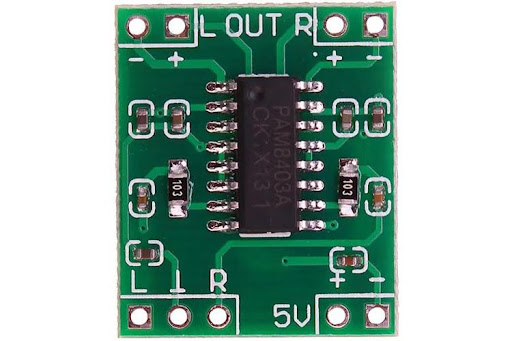
\includegraphics[width=0.3\linewidth]{assets/ch2/PAM8403}
		\caption{PAM8403 Audio Amplification Module}
		\label{fig:pam8403}
	\end{figure}
	
	
	\item \textbf{TPA3116D2}: A powerful audio amplifier capable of delivering higher output power, often used in larger audio systems.
	
	\begin{figure}[h!]
		\centering
		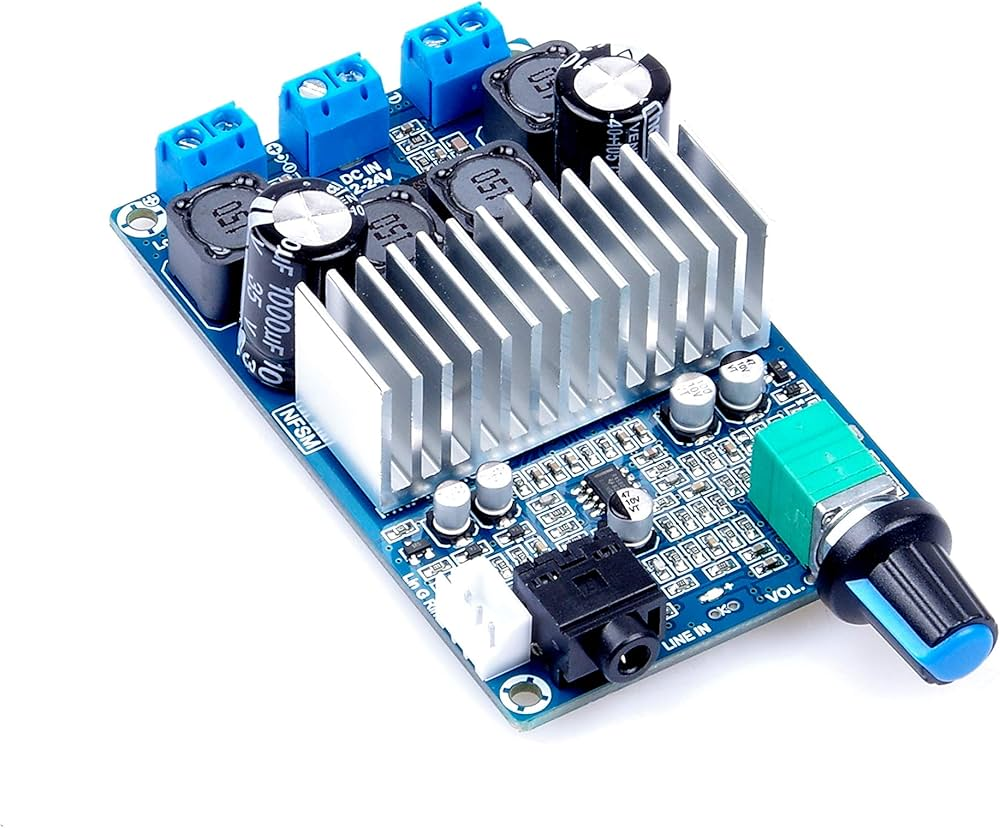
\includegraphics[width=0.3\linewidth]{assets/ch2/TPA3116D2}
		\caption{TPA3116D2 Audio Amplification Module}
		\label{fig:tpa3116d2}
	\end{figure}
	
	\item \textbf{LM386}: A low-power audio amplifier that is easy to use and perfect for basic applications.
	\begin{figure}[h!]
		\centering
		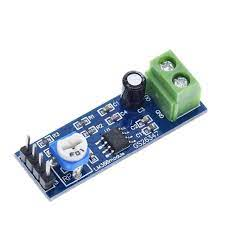
\includegraphics[width=0.3\linewidth]{assets/ch2/LM386}
		\caption{LM386 Audio Amplification Module}
		\label{fig:lm386}
	\end{figure}
	
	\item \textbf{MAX9744}: A high-efficiency audio amplifier designed for demanding audio applications, providing high-quality sound output.
	\begin{figure}[h!]
		\centering
		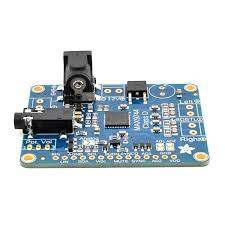
\includegraphics[width=0.3\linewidth]{assets/ch2/MAX9744}
		\caption{MAX9744 Audio Amplification Module}
		\label{fig:max9744}
	\end{figure}
	
\end{itemize}
